
\documentclass[a4paper, 12pt]{book}

% XXX: why utf8x and not utf8?
\usepackage[utf8x]{inputenc}   % omogoča uporabo slovenskih črk v UTF-8

\usepackage[slovene,english]{babel}  % slovenski delilni vzorci ipd.
\usepackage[pdftex]{graphicx}  % omogoča vlaganje slik različnih formatov 
\usepackage{fancyhdr}          % poskrbi, na primer, za glave strani
\usepackage{amssymb}           % dodatni simboli
\usepackage{amsmath}
\usepackage{fixltx2e}          % textsubscript etc. (XXX: used anywhere here?)
\usepackage{color}
\usepackage{array}
\usepackage{tabulary}
\usepackage{icomma}            % comma as a decimal separator

\usepackage{pgfplots}

\usepackage{numprint}          % number formating
\npthousandsep{.}\npthousandthpartsep{}\npdecimalsign{,}

\usepackage[lined,plain,linesnumbered]{algorithm2e}
\usepackage{setspace}

% reduce line spacing for algorithms to save space
\usepackage{etoolbox}
\AtBeginEnvironment{algorithm}{\setstretch{1.05}\small}

% change algorithm label name
\renewcommand{\algorithmcfname}{Psevdokoda}



\renewcommand*{\familydefault}{\rmdefault}  % default font family (roman)
\renewcommand{\baselinestretch}{1.3}  % ustrezen razmik med vrsticami

\renewcommand{\arraystretch}{1.3}  % razmik med vrsticami tabel
\AtBeginEnvironment{tabular}{\small}

%oznake strani
\renewcommand{\chaptermark}[1]%
{\markboth{\MakeUppercase{\thechapter.\ #1}}{}}
\renewcommand{\sectionmark}[1]%
{\markright{\MakeUppercase{\thesection.\ #1}}}
\renewcommand{\headrulewidth}{0.5pt} \renewcommand{\footrulewidth}{0pt}
\fancyhf{}
\fancyhead[LE,RO]{\sl \thepage} \fancyhead[LO]{\sl \rightmark}
\fancyhead[RE]{\sl \leftmark}

\newcommand{\BibTeX}{{\sc Bib}\TeX}

\newcommand{\autfont}{\Large}
\newcommand{\titfont}{\LARGE\bf}
\newcommand{\newterm}{\textit}

%\newcommand{\TODO}{\textcolor{red}}
\newcommand{\TODO}[1]{\textcolor{red}{(TODO: #1)}}
\newcommand{\sub}{\textsubscript}

\newcommand{\clearemptydoublepage}{
	\newpage{\pagestyle{empty}\cleardoublepage}}
\setcounter{tocdepth}{2}	      % globina kazala

% konstrukti
\newtheorem{izrek}{Izrek}[chapter]

%\newtheorem{trditev}{Trditev}[izrek]
\newenvironment{dokaz}{\emph{Dokaz.}\ }{\hspace{\fill}{$\Box$}}

\newenvironment{itquote}
{\begin{quote}\itshape}
{\end{quote}}

\begin{document}
\selectlanguage{slovene}
\frontmatter
\setcounter{page}{1} %
\renewcommand{\thepage}{}  % preprecimo težave s številkami strani v kazalu


%%%%%%%%%%%%%%%%%%%%%%%%%%%%%%%%%%%%%%%%
%naslovnica
\label{naslovnica}
\thispagestyle{empty}%
\begin{center}
    {\large\sc Univerza v Ljubljani\\%
      Fakulteta za računalništvo in informatiko}%
    \vskip 10em%
    {\autfont Peter Lamut\par}%
    {\titfont \TODO{Naslov diplomskega dela} \par}%
    {\vskip 2em \textsc{DIPLOMSKO DELO NA UNIVERZITETNEM ŠTUDIJU
    RAČUNALNIŠTVA IN INFORMATIKE}\par}%
    \vfill\null%
    {\large \textsc{Mentor}: doc.\ dr. Boštjan Slivnik\par}%
    {\vskip 2em \large Ljubljana 2014 \par}%
\end{center}

% prazna stran
\clearemptydoublepage


%%%%%%%%%%%%%%%%%%%%%%%%%%%%%%%%%%%%%%%%
%copyright stran
\label{copyright_page}
\thispagestyle{empty}
\vspace*{8cm}

{\small \noindent
Rezultati diplomskega dela so intelektualna lastnina avtorja in Fakultete za
ra\-ču\-nal\-niš\-tvo in informatiko Univerze v Ljubljani.
Za objavljanje ali izkoriščanje rezultatov di\-plom\-ske\-ga dela je potrebno
pisno soglasje avtorja, Fakultete za ra\-ču\-nal\-niš\-tvo in
informatiko ter mentorja.}%
\footnote{V dogovoru z mentorjem lahko kandidat diplomsko delo s pripadajočo
izvorno kodo izda tudi pod katero izmed alternativnih licenc, ki ponuja
določen del pravic vsem: npr. Creative Commons, GNU GPL. V tem primeru na to
mesto vstavite opis licence, na primer tekst \cite{licence}

 \TODO{Morda pa res raje izdaj pod katero izmed prostih licenc?}
}


\begin{center} 
\mbox{}\vfill
% TODO: a je to potrebno tukaj? kje drugje morda?
\emph{Besedilo je oblikovano z urejevalnikom besedil \LaTeX.} 
\end{center}


% prazna stran
\clearemptydoublepage


%%%%%%%%%%%%%%%%%%%%%%%%%%%%%%%%%%%%%%%%
% stran 3 med uvodnimi listi
\noindent
\TODO{Namesto te strani {\bf vstavite} original izdane teme diplomskega 
dela s podpisom mentorja in dekana ter žigom fakultete, ki ga diplomant
dvigne v študent\-skem referatu,  preden odda izdelek v vezavo!
Glej tudi sam konec Poglavja~\ref{ch2} na strani~\pageref{pp}.}

% prazna stran
\clearemptydoublepage


%%%%%%%%%%%%%%%%%%%%%%%%%%%%%%%%%%%%%%%%
% izjava o avtorstvu
\label{izjava_avtorstvo}

\vspace*{1cm}
\begin{center} 
{\Large \textbf{\sc Izjava o avtorstvu diplomskega dela}}
\end{center}

\vspace{1cm}
\noindent Spodaj podpisani Peter Lamut,
z vpisno številko \textbf{63000200}, sem avtor diplomskega dela z naslovom:
   
\vspace{0.5cm}
\emph{\TODO{naslov diplomskega dela}}

\vspace{1.5cm}
\noindent S svojim podpisom zagotavljam, da:

\begin{itemize}
	\item sem diplomsko delo izdelal samostojno pod mentorstvom 
		doc.\ dr.\ Boštjana Slivnika,

	\item so elektronska oblika diplomskega dela, naslov (slov., angl.),
	 povzetek (slov., angl.) ter ključne besede (slov., angl.) identični
	 s tiskano obliko diplomskega dela,
	
	\item soglašam z javno objavo elektronske oblike diplomskega dela
	v zbirki ``Dela FRI''.
\end{itemize}

\vspace{1cm}

\noindent V Ljubljani, dne \TODO{datum, npr. 1. aprila 2014} \hfill
Podpis avtorja:

% prazna stran
\clearemptydoublepage


%%%%%%%%%%%%%%%%%%%%%%%%%%%%%%%%%%%%%%%%
% zahvala

\label{zahvala}
\thispagestyle{empty}\mbox{}\vfill\null\it%
\TODO{Na tem mestu zapišite, komu se zahvaljujete za izdelavo diplomske
naloge. Pazite, da ne boste koga pozabili. Utegnil vam bo zameriti. Temu
se da izogniti tako, da pozabite na celo zahvalo.}
\rm\normalfont

% prazna stran
\clearemptydoublepage


%%%%%%%%%%%%%%%%%%%%%%%%%%%%%%%%%%%%%%%%
% kazalo
\label{kazalo}
\def\thepage{}% preprecimo tezave s stevilkami strani v kazalu 
\tableofcontents{}


% prazna stran
\clearemptydoublepage


%%%%%%%%%%%%%%%%%%%%%%%%%%%%%%%%%%%%%%%%
% povzetek
% TODO: napiši na koncu
\addcontentsline{toc}{chapter}{Povzetek}
\chapter*{Povzetek}

\TODO{Ključne besede:}%

\TODO{V vzorcu je predstavljen postopek priprave diplomskega dela z uporabo
okolja \LaTeX. Vaš povzetek mora sicer vsebovati približno 100 besed, ta
tukaj je odločno prekratek.}

% prazna stran
\clearemptydoublepage


%%%%%%%%%%%%%%%%%%%%%%%%%%%%%%%%%%%%%%%%
% abstract
\selectlanguage{english}
\addcontentsline{toc}{chapter}{Abstract}
\chapter*{Abstract}

\TODO{Keywords:}

\TODO{This sample document presents an approach to typesetting your BSc
thesis using \LaTeX. A proper abstract should contain around 100 words which
makes this one way too short.}

\selectlanguage{slovene}

% prazna stran
\clearemptydoublepage


%%%%%%%%%%%%%%%%%%%%%%%%%%%%%%%%%%%%%%%%
\mainmatter
\setcounter{page}{1}
\pagestyle{fancy}

\chapter{Uvod}

\section{Splošno o podatkovnih omrežjih}

\TODO{slovenski términ za datagrid pravilen?}

Podatkovno omrežje (angl. \textit{datagrid}) je množica med seboj
povezanih računalnikov na različnih geografskih lokacijah, ki uporabnikom
omogočajo nalaganje, hranjenje in medsebojno izmenjavanje datotek.
(TODO: vir definicije / ustrezno prilagodi definicijo)

\TODO{Omeni, da imaš različne topologije, da je cilj robustnost, redundanca,
itd., sklicuj se pač na vire - odstavek ali dva max. (1 stran)}

\TODO{Pa morda še kakšna slika kot primer (nariši npr. z LaTeXom - kar tako,
 za vajo)}

\section{Replikacija podatkov v podatkovnih omrežjih}

Ko uporabnik podatkovnega omrežja pošlje zahtevek za prejem neke datoteke
ali skupine datotek, se lahko pri prenašanju podatkov od glavnega strežnika
do odjemalca porabi veliko pasovne širine. Poleg tega je lahko tudi čas,
potreben za prenos, dolg. Zaradi tega je morda smiselno za posamezno
datoteko ustvariti več njenih kopij na različnih lokacijah v omrežju.
Tovrstne kopije datotek imenujemo \newterm{replike}.

Cilj ustvarjanja replik je zmanjšati porabo pasovne širine in izboljšati
odzivne čase podatkovnega omrežja (\TODO{vir, kjer sta omenjena ta dva
cilja}). Če je neka replika na voljo tudi lokalno (bliže
uporabniku, ki jo zahteva), je namreč ni potrebno vsakič znova prenašati s
strežnika, temveč se preprosto uporabi lokalna kopija.

Posamezna vozlišča (računalniki) v omrežju praviloma nimajo dovolj prostora,
da bi hranila vse replike naenkrat. Zaradi te omejitve je potrebna
strategija, na podlagi katere se odločimo, katere replike bomo hranili
na katerih vozliščih --- seveda tako, da bo zadani cilj (\TODO{številčna
referenca prej opisanega cilja?}) čim bolje izpolnjen.

Replikacijske strategije ločimo v dve skupini, in sicer poznamo
\newterm{statično replikacijo} in \newterm{dinamično replikacijo}
(\TODO{viri, kjer je to navedeno}).

\subsection{Statična replikacija}

Pri statični replikaciji za vsako posamezno vozlišče že vnaprej določimo,
katere replike bodo shranjene na njem. Problem, kako replike čim bolje
razporediti po omrežju, lahko obravnavamo kot statičen optimizacijski
problem. Zanj se sicer izkaže, da je tako NP-težek kot tudi
neaproksimativen.

\TODO{referenca kakšnega članka, ki o tem govori, npr. Čibej}

\subsection{Dinamična replikacija}

Pri dinamični replikaciji se vsako vozlišče avtonomno odloča, katere
replike bo hranilo, pri čemer se lahko množica shranjenih replik na
posameznem vozlišču skozi čas spreminja. Če vozlišče na podlagi neke
metrike oceni, da je pravkar zahtevana replika zanj bolj pomembna od ene
ali več obstoječih shranjenih replik, lahko slednje izbriše in namesto
njih shrani novo repliko.

Dinamična replikacija je boljša od statične, saj se lahko avtomatično
prilagaja morebitnim spremembam v vzorcih uporabe podatkovnega omrežja
\TODO{citat Čibej}. Poznamo veliko različnih dinamičnih replikacijskih
strategij, pri čemer je ena izmed najbolj učinkovitih algoritem
\newterm{Fast Spread} (\TODO{vir -- Ranganathan and Foster, 2001b?}).

\TODO{Fast spread prevedemo v slovenščino? ``algoritem hitrega širjenja''?}


\section{Algoritem Fast Spread}

Algoritem Fast Spread se uporablja v hierarhično urejenih podatkovnih omrežjih.
Na vrhu hierarhije je glavni strežnik, ki ima dovolj prostora, da vedno hrani
vse replike, ki obstajajo v omrežju. V primerjavi z njim je prostor na vseh
ostalih vozliščih relativno majhen, tako da lahko slednja naenkrat hranijo
zgolj omejeno podmnožico replik. Vozlišča so lahko poljubno povezana med seboj
in ni nujno, da ima vsako izmed njih neposredno povezavo z glavnim strežnikom
-- z njim so lahko povezana tudi zgolj posredno preko drugih vozlišč.

Za vsako vozlišče v omrežju obstaja najkrajša pot do strežnika in vsako izmed
njih ve, katero vozlišče je njihov starš na tej poti. Kadar vozlišče prejme
zahtevek za določeno repliko in slednje nima shranjene lokalno, zahtevek
posreduje svojemu staršu, ta pa lahko isti zahtevek posreduje še naprej
navzgor po hierarhiji, dokler ga ne prejme vozlišče, ki repliko ima. Če ne
prej, se to zgodi takrat, ko zahtevek prispe do glavnega strežnika.

\TODO{kakšna lepa slikica?}

Prvo vozlišče v verigi, ki najde zahtevano repliko pri sebi, le-to pošlje
vozlišču, ki jo je od njega zahtevalo. Slednje jo nato posreduje še naprej
navzdol po hierarhiji, dokler replika ne prispe do vozlišča, ki je poslalo
prvotni zahtevek zanjo. Pri tem vsako izmed vozlišč na poti repliko tudi
lokalno shrani.

V primeru, da določeno vozlišče nima dovolj prostora, da bi shranilo repliko,
mora predhodno izbrisati eno ali več obstoječih replik. Katere izmed njih bodo
zamenjane z novo repliko, je odvisno od tega, katero strategijo zamenjave
uporablja vozlišče. Poznamo veliko različnih strategij, npr.
\TODO{morda naštej nekaj?}. Izmed njih bom opisal dve, ki so jih avtorji
člankov \TODO{referenca?} uporabili za primerjavo s strategijama, ki so ju
predlagali sami.

\TODO{kakšna referenca na vir, ki Fast Spread opisuje?}

\subsection{Strategija zamenjave LRU}

Pri strategiji \newterm{LRU} (\newterm{``Least Recently Used"}) vozlišče
zamenja tisto repliko (ali skupino replik), pri kateri je preteklo največ
časa od prejema zadnjega zahtevka zanjo --- torej tisto, ki najdlje časa
ni bila uporabljena.

\subsection{Strategija zamenjave LFU}

Pri strategiji \newterm{LFU} (\newterm{``Least Frequently Used"}) vozlišče
zamenja tisto repliko (ali skupino replik), ki je bila v preteklosti
najmanjkrat zahtevana. Strategija torej upošteva vse pretekle zahtevke za
posamezno repliko in ne zgolj zadnjega, kot je to pri strategiji LRU.

\section{Trditev v člankih: izboljšava algoritma Fast Spread}

Leta 2011 in 2012 sta bila v dveh različnih strokovnih revijah objavljena
dva članka istih avtorjev, v katerih so slednji predstavili dve novi
strategiji zamenjave, ki naj bi po njihovih trditvah dosegali dosti boljše
rezultate od strategij LRU in LFU. Strategiji
so poimenovali \newterm{EFS} (\newterm{``Enhanced Fast Spread''}) in
\newterm{MFS} (\newterm{``Modified Fast Spread''})
\TODO{vir oz. referenca člankov}.

\TODO{oštevilči članka? Da se kasneje v besedilu sklicuješ nanj? Kako se
to ponavadi dela?}

Članka sta si med seboj že na prvi pogled zelo podobna. Oba imata identično
strukturo (identične naslove posameznih delov članka), vsebujeta številne
identične odseke besedila, identične diagrame in tudi opisa obeh strategij
v psevdokodi sta v veliki meri enaka. Na podlagi naštetega se je pojavil
resen sum na recikliranje člankov (avtoplagiatorstvo).

\TODO{vstavi slike, dele besedila itd. za primerjavo pa to omeni v tekstu}

V okviru diplomskega dela sem z implementacijo strategij, opisanih v
člankih, želel doseči predvsem naslednje cilje:
\label{cilji}

\begin{enumerate}
\item Preveriti rezultate, ki so jih dosegli avtorji člankov.

\item Neposredno primerjati strategiji iz člankov \TODO{2011} in
\TODO{2012} med seboj. V obeh člankih namreč avtorji v njih opisani
strategiji primerjajo zgolj s strategijama LRU in LFU, medsebojne
primerjave pa v novejšem članku (\TODO{2012}) niso naredili.

\item Na podlagi primerjave obeh opisanih strategij ugotoviti, ali med
člankoma sploh obstaja kakšna bistvena vsebinska razlika.
\end{enumerate}


\chapter{Primerjava strategij iz člankov}

\section{Opis strategij zamenjave}
Kot je že bilo omenjeno (\TODO{v poglacju XYZ?}), algoritem Fast Spread
shrani zahtevano repliko na vsakem vozlišču na poti od vozlišča, kjer je
bila zahtevana replika najdena, do vozlišča, ki je repliko prvotno
zahtevalo. Če določeno vozlišče nima dovolj razpoložljivega prostora,
da bi zahtevano repliko shranilo, mora najprej izbrisati eno ali več
obstoječih replik.

Avtorji člankov (\TODO{št. oznaka člankov?}) opozarjajo, da je lahko
skupina replik, ki jih je potrebno izbrisati, ``bolj pomembna" od
nove replike. Izpostavljajo, da algoritem Fast Spread tega ne upošteva in
da zamenjavo skupine obstoječih replik z novo repliko vedno
izvede ne glede na morebitno večjo vrednost skupine replik
(\TODO{sklic na ustrezen del članka - oz. v obeh}).

Avtorji v obeh člankih predlagajo nekoliko spremenjeni različici algoritma
Fast Spread, ki izvedeta zamenjavo le v primerih, ko je vrednost skupine
replik strogo manjša od vrednosti nove replike. Pri tem algoritma za
ocenjevanje vrednosti (skupin) replik uporabljata metrike, opisane v
nadaljevanju.

\subsection{Strategija EFS}

Psevdokoda strategije EFS je prikazana na Sliki~\ref{alg:EFS}, pri čemer
je pomen posameznih spremenljivk pojasnjen v Tabeli~\ref{tbl:EFS_vars}.

\begin{algorithm}
  \label{alg:EFS}
  \caption{Strategija EFS (\TODO{preimenuj bold oznako + referenca
  na članek})}

  \SetKwComment{blankln}{}{}

  Initialize SOS to $0$\;
  \eIf{RR exists on RN}{
      Use RR\;
  }{
      \For{$i = 2$ \KwTo NSPList.size}{
          \If{RR exists on NSPList(i)}{
              \For{$j = \mathit{NSPList}(i - 1)$ \KwTo $1$}{
                  \eIf{CNFSS $\geq$ RR.Size}{
                      Copy RR\;
                  }{
                      \For{$x = 1$ \KwTo ReplicaList.size}{
                          \eIf{$\mathit{SOS} + \mathit{CNFSS} <$ RR.Size}{
                              SOS = SOS + \textit{SizeList(x)}\;
                          }{
                              Break\;
                          }
                      }

\blankln{}

                      $\mathit{GV} = \frac{\sum_{y=1}^{x-1}
                          \mathit{NORList(y)}}{
                                  \sum_{y=1}^{x-1} \mathit{SizeList(y)}} +
                          \frac{\sum_{y=1}^{x-1}
                              \mathit{NORFSTIList(y)}}{\mathit{FSTI}} +
                          \frac{1}{\mathit{CT} - \frac{\sum_{y=1}^{x-1}
                              \mathit{LRTList(y)}}{x-1}}$

\blankln{}

                      $\mathit{RV_{RR}} =
                          \frac{\mathit{NORRR}}{\mathit{SRR}} +
                          \frac{\mathit{NORRRFSTI}}{\mathit{FSTI}} +
                          \frac{1}{\mathit{CT} - \mathit{LRTRR}}$

\blankln{}

                      \If{$\mathit{GV} < \mathit{RV_{RR}}$} {
                          \For{$y = 1$ \KwTo $x-1$}{
                            Delete \textit{ReplicaList(y)},
							  \textit{NORList(y)},
							  \textit{SizeList(y)}, \textit{NORFSTIList(y)},
							  \textit{LRTList(y)}\;
                          }
                          Copy RR;
                      }
                  }
              }
          }
      }
  }
\end{algorithm}

\begin{table}
\small
  \begin{center}
    \begin{tabulary}{1.0\textwidth}{ >{\itshape}p{7em} J}
      \textnormal{Spremenljivka} & Pomen \\
      \hline
      RR & zahtevana replika \\
      RN &  vozlišče, ki zahteva repliko \\
      CNFSS & nezaseden prostor na trenutno opazovanem vozlišču \\
      FSTI & frekvenčno-specifičen časovni razpon \TODO{prevod???} \\
      NORRR & število zahtevkov za \textit{RR} \\
      SRR & velikost \textit{RR} \\
      NORRRFSTI & število zahtevkov za zahtevano repliko
          v \textit{FSTI} \\
      CT & trenutni čas \\
      LRTRR & čas zadnjega zahtevka za zahtevano repliko \\
      SOS & spremenljivka, ki predstavlja vsoto velikosti skupine replik na
          trenutno opazovanem vozlišču \\
      NSPList & seznam vozlišč na najkrajši poti od \textit{RN} do
          glavnega strežnika \\
      ReplicaList & seznam obstoječih replik na trenutno opazovanem vozlišču,
          urejenih po naraščajočem vrstnem redu glede na njihovo vrednost
          \textit{RV}. Če ima več replik enako vrednost \textit{RV}, so med
          seboj urejene naključno. \\
      NORList & seznam, ki vsebuje vrednosti, kolikokrat so bile istoležne
          replike s seznama \textit{ReplicaList} zahtevane s strani
          trenutno opazovanega vozlišča. \\
      SizeList & seznam, ki vsebuje velikosti istoležnih replik s seznama
          \textit{ReplicaList} \\
      NORFSTIList & seznam, ki vsebuje vrednosti, kolikokrat so bile istoležne
          replike s seznama \textit{ReplicaList} zahtevane v \textit{FSTI} s
          strani trenutno opazovanega vozlišča \\
      LRTList & seznam, ki vsebuje čase zadnjega zahtevka za istoležne
          replike s seznama \textit{ReplicaList}
    \end{tabulary}
 \end{center}

  \caption{Pomen spremenljivk v psevdokodi algoritma EFS.}
  \label{tbl:EFS_vars}
\end{table}

Kadar neko vozlišče prejme zahtevano repliko, za shranitev katere nima dovolj
nezasedenega prostora (\TODO{ref. vrstica 10}), pogleda, koliko
obstoječih replik bi zaradi tega moralo predhodno izbrisati. Sprehodi se skozi
seznam~\textit{\mbox{ReplicaList}}, dokler vsota velikosti obiskanih replik in
velikosti nezasedenega prostora ne doseže (ali preseže) velikosti nove replike
(\TODO{referenca vrstice 11--17}). Vse obiskane replike nato implicitno
tvorijo skupino replik, ki bodo potencialno izbrisane.

Vozlišče v nadaljevanju izračuna vrednosti nove replike in skupine replik
(vrstici 18 in 19 \TODO{ref.}) ter ju med seboj primerja. V primeru, da je
vrednost skupine manjša (vrstica 20 \TODO{}), vozlišče izbriše vse replike
iz skupine in njihove statistike ter jih nadomesti z novo repliko
(vrstice 21--24 \TODO{ref.}).

Strategija EFS pri ocenjevanju vrednosti replik upošteva naslednje štiri
stvari:

\begin{itemize}
  \item število zahtevkov za repliko,
  \item pogostost zahtevkov,
  \item velikost replike,
  \item čas od zadnjega zahtevka za repliko.
\end{itemize}

\TODO{item spacing too big}

Število zahtevkov, njihova pogostost in čas od zadnjega zahtevka so pomembni
dejavniki, saj z njihovo pomočjo lahko ocenimo verjetnost, da bo replika
v prihodnosti ponovno zahtevana. Ker imajo vozlišča omejen prostor za
shranjevanje replik, je pomembna tudi velikost slednjih
\TODO{referenca na članek 2011}.

\begin{samepage}
Iz vrstice 19 (\TODO{referenca}) psevdokode \TODO{sklic} lahko razberemo
formulo za izračun vrednosti posamezne replike:
\begin{equation}
  \mathit{RV} = \frac{\mathit{NORRR}}{\mathit{SRR}} +
                      \frac{\mathit{NORRRFSTI}}{\mathit{FSTI}} +
                      \frac{1}{\mathit{CT} - \mathit{LRTRR}}
  \label{eq:EFS_RV}
\end{equation}
pri čemer je pomen posameznih spremenljivk pojasnjen v
Tabeli~\ref{tbl:EFS_vars}.
\end{samepage}

Iz prvega in drugega člena enačbe~\eqref{eq:EFS_RV} je razvidno, da imajo
višjo vrednost tiste replike, ki so bile večkrat zahtevane (večje število
zahtevkov), pri čemer drugi člen upošteva zgolj zahtevke iz nedavne zgodovine,
torej znotraj intervala FSTI, ki jih dodatno normira z velikostjo tega
intervala. Iz prvega člena je tudi razvidno, da je vrednost replik obratno
sorazmerna z njihovo velikostjo. Večje replike so vrednotene niže, saj
zasedajo več prostora na vozlišču. Zadnji člen daje višjo vrednost replikam,
katerih čas od njihovega zadnjega zahtevka je manjši.

\TODO{zdaj pa še group value pojasni}

\begin{samepage}
Podobno kot vrednost posamezne replike se izračuna tudi vrednost skupine
replik, in sicer po formuli iz vrstice 18 \TODO{} v
\TODO{EFS psevdokoda referenca}:
\begin{equation}
  \mathit{GV} = \frac{\sum\limits_{y=1}^{x-1} \mathit{NORList(y)}}{
                      \sum\limits_{y=1}^{x-1} \mathit{SizeList(y)}} +
                \frac{\sum\limits_{y=1}^{x-1} \mathit{NORFSTIList(y)}}{
                      \mathit{FSTI}} +
                \frac{1}{\mathit{CT} - \frac{\sum\limits_{y=1}^{x-1}
                         \mathit{LRTList(y)}}{x-1}}
  \label{eq:EFS_GV}
\end{equation}
pri čemer je pomen posameznih spremenljivk pojasnjen v
Tabeli~\ref{tbl:EFS_vars}.
\end{samepage}

Enačbi~\eqref{eq:EFS_RV}~in~\eqref{eq:EFS_GV} sta vsebinsko gledano
pravzaprav enaki. Edina razlika je, da so posamezni členi iz
enačbe~\eqref{eq:EFS_RV} v enačbi~\eqref{eq:EFS_GV} namesto za posamezno
repliko izračunani na ravni celotne skupine replik.
Tako je med drugim v prvem členu enačbe~\eqref{eq:EFS_GV} izračunano razmerje
med skupnim številom zahtevkov in skupno velikostjo \textit{vseh replik} iz
skupine, v tretjem členu pa je uporabljen \textit{povprečen čas} od zadnjega
zahtevka za posamezno repliko v skupini.

\TODO{a bi v GV morali deliti 2. člen še s številom replik v skupini?
Konceptualno gledano verjetno da, ampak v članku to ni tako navedeno) ---
na to opozori pri razpravi o članku}


\subsection{Strategija MFS}

Strategija MFS (psevdokoda na Sliki~\ref{alg:MFS})
je konceptualno popolnoma enaka strategiji EFS. Od nje se razlikuje
zgolj v formulah za izračun vrednosti replike in vrednosti skupine replik
ter v načinu, na katerega so replike urejene v seznamu \textit{ReplicaList}.

\begin{samepage}
Vrednost replike se izračuna po naslednji formuli iz vrstice 11
(\TODO{ref.}) v Psevdokodi~\ref{alg:MFS}:
\begin{equation}
  \mathit{PNOR} = \mathit{NOR} \times
                  \frac{\mathit{RR.Size} - \mathit{CNFSS}}{
                        \mathit{ RR.Size}}
  \label{eq:MFS_RV}
\end{equation}
pri čemer je pomen posameznih spremenljivk pojasnjen v
Tabeli~\ref{tbl:MFS_vars}.
\end{samepage}

Vrednost replike je PNOR oziroma ``delno število zahtevkov''. Izračuna
se kot skupno število zahtevkov za repliko (NOR), prilagojeno za
korekcijski faktor. Slednji je odvisen od razmerja med velikostjo replike
in velikostjo nezasedenega prostora na vozlišču. V robnem primeru,
ko je ves razpoložljiv prostor na vozlišču zaseden (CNFSS je enak 0), sta
vrednosti PNOR in NOR enaki. PNOR ni nikoli negativno število.%
\footnote{Ulomek v enačbi~\eqref{eq:MFS_RV} je vedno pozitiven, saj
je njegov imenovalec pozitiven -- velikost replike \textit{RR.Size} je
namreč strogo večja od velikosti nezasedenega prostora \textit{CNFSS}. Če
bi bilo obratno, bi namreč vozlišče repliko takoj shranilo in niti ne bi
šlo računati njene vrednosti, kar je razvidno iz vrstic 8 in 9
 \TODO{(ref.)} v Psevdokodi~\ref{alg:MFS}.}



\begin{samepage}
Vrednost skupine replik se izračuna po formuli, ki se nahaja na levi strani
neenakosti v vrstici 18 (\TODO{ref.}) Psevdokode~\ref{alg:MFS}:
\begin{equation}
	\sum\limits_{y=1}^{x-1} \mathit{NORList(y)}
  \label{eq:MFS_GV}
\end{equation}
pri čemer je pomen posameznih spremenljivk pojasnjen v
Tabeli~\ref{tbl:MFS_vars}.
\end{samepage}

Formula~\eqref{eq:MFS_GV} je zelo enostavna, saj zgolj sešteje število
zahtevkov (NOR) za vse replike, ki sestavljajo skupino.

Kot že omenjeno se strategija MFS od strategije EFS nekoliko razlikuje
tudi v tem, iz katerih replik vozlišče sestavi skupino replik, ki bodo morda
zamenjane. Razlog za to je različna urejenost replik v seznamu
\textit{ReplicaList}. Medtem ko strategija EFS replike uredi glede na
njihovo vrednost (RV), jih strategija MFS uredi glede na
število zahtevkov zanje, v primeru enakih vrednosti pa še dodatno
glede na njihovo velikost. Urejenosti seznama \textit{ReplicaList} je
sicer opisana tudi v Tabelah~\ref{tbl:EFS_vars}~oziroma~\ref{tbl:MFS_vars}.

\TODO{pseudocode vertical spacing?}

\begin{algorithm}[H]
  \label{alg:MFS}
  \caption{Strategija MFS (\TODO{preimenuj bold oznako + referenca
  na članek})}

  \SetKwComment{blankln}{}{}

  Initialize SOS to $0$\;
  \eIf{RR exists on RN}{
      Use RR\;
  }{
      \For{$i = 2$ \KwTo NSPList.size}{
          \If{RR exists on NSPList(i)}{
              \For{$j = \mathit{NSPList}(i - 1)$ \KwTo $1$}{
                  \eIf{CNFSS $\geq$ RR.Size}{
                      Copy RR\;
                  }{
                      $\mathit{PNOR} =
                          \mathit{NOR} \times
                          \tfrac{\mathit{RR.Size} - \mathit{CNFSS}}{
                                 \mathit{ RR.Size}}$

                      \For{$x = 1$ \KwTo ReplicaList.size}{
                          \eIf{SOS $<$ RR.Size $- \mathit{CNFSS}$}{
                              SOS = SOS + \textit{SizeList(x)}\;
                          }{
                              Break\;
                          }
                      }

                      \If{$\sum_{y=1}^{x-1} \mathit{NORList(y)} <
                          \mathit{PNOR}$} {
                          \For{$y = 1$ \KwTo $x-1$}{
                              Delete \textit{ReplicaList(y)},
                              \textit{SizeList(y)}, \textit{NORList(y)}\;
                          }
                          Copy RR;
                      }
                  }
              }
          }
      }
  }
\end{algorithm}


\begin{table}
\small
  \begin{center}
    \begin{tabulary}{1.0\textwidth}{ >{\itshape}p{7em} J}
      \textnormal{Spremenljivka} & Pomen \\
      \hline
      RR & zahtevana replika \\
      RN &  vozlišče, ki zahteva repliko \\
      CNFSS & nezaseden prostor na trenutno opazovanem vozlišču \\
      NOR & število zahtevkov za \textit{RR} \\
      PNOR & delno število zahtevkov za \textit{RR} \\
      SOS & spremenljivka, ki predstavlja vsoto velikosti skupine replik na
          trenutno opazovanem vozlišču \\
      NSPList & seznam vozlišč na najkrajši poti od \textit{RN} do
          glavnega strežnika \\
      ReplicaList & seznam obstoječih replik na trenutno opazovanem vozlišču,
          urejenih po naraščajočem vrstnem redu glede na njihovo vrednost
          \textit{NOR}.
          Če ima več replik enako vrednost \textit{NOR}, so slednje med seboj
          urejene v padajočem vrstnem redu glede na njihovo velikost. Če so
          tudi velikosti enake, je medsebojni vrstni red teh replik
          naključen. \\
      SizeList & seznam, ki vsebuje velikosti istoležnih replik s seznama
          \textit{ReplicaList} \\
      NORList & seznam, ki vsebuje vrednosti, kolikokrat so bile istoležne
          replike s seznama \textit{ReplicaList} zahtevane s strani
          trenutno opazovanega vozlišča. \\
    \end{tabulary}
  \end{center}

  \caption{Pomen spremenljivk v psevdokodi algoritma MFS.}
  \label{tbl:MFS_vars}
\end{table}

\TODO{force table and to be under the Strategija MFS
section?}

\TODO{strategija Fast Spread with EFS / MFS - kakšne reference na članke, kjer
sta strategiji opisani?}


\section{Implementacija diskretne simulacije}

Za preizkus strategij, opisanih v člankih, sem v programskem jeziku Python
(različica 3.3) napisal diskretno simulacijo. S poganjanjem slednje z
različnimi parametri sem lahko primerjal, kako se obnesejo posamezne strategije
zamenjave. Glavni sestavni deli simulacije so vozlišča, replike, dogodki v
simulaciji in sámo izvajalno okolje simulacije.
\TODO{link na Github, kjer je koda? morda koda kot priloga diplome?}

Topologija podatkovnega omrežja, ki sem jo uporabil, je polni graf, saj so
takšno topologijo izbrali tudi avtorji člankov \TODO{referenca obeh čl.}.
Povezave med vsakim parom vozlišč so simetrične, njihove dolžine pa se v fazi
inicializacije simulacije naključno določijo. V isti fazi se generirajo tudi
replike naključnih velikosti.

Ko so dolžine povezav med vozlišči določene, se na grafu, ki predstavlja
podatkovno omrežje, izvede algoritem Dijkstra, ki poišče najkrajše poti med
glavnim strežnikom in vsemi ostalimi vozlišči. Po izvedbi algoritma vsakemu
vozlišču določimo, kdo je njegov starš na najkrajši poti do glavnega strežnika%
\footnote{Sam glavni strežnik je pri tem seveda izjema, saj se nahaja povsem
na vrhu hierarhije in starša nima.}.

Med izvajanjem simulacije je vsako vozlišče avtonomno in se samo odloča, katere
replike bo hranilo pri sebi, pri čemer sledi vnaprej določeni strategiji
zamenjave. V posamezni izvedbi simulacije vsa vozlišča uporabljajo enako
strategijo in je med izvajanjem ne spreminjajo.

\subsection{Vrste dogodkov v simulaciji}
V okviru simulacije so definirane naslednje štiri vrste dogodkov, ki se lahko
pojavijo v njej:
\begin{itemize}
  \item \textbf{Pošlji zahtevek za repliko:} Vozlišče svojemu staršu pošlje
  zahtevek za repliko, ki je sámo nima. Posledično se za starša po določeni
  zakasnitvi sproži dogodek \textit{prejmi zahtevek za repliko}.

  \item \textbf{Prejmi zahtevek za repliko:} Vozlišče prejme zahtevek za
  določeno repliko od enega izmed svojih sinov. Če repliko ima, sproži dogodek
  \textit{pošlji repliko}, sicer pa posreduje zahtevek za isto repliko
  naprej svojemu staršu in s tem sproži dogodek \textit{pošlji zahtevek za
  repliko}.

  Če vir zahtevka ni določen, to označuje, da je zahtevek ustvarilo kar
  vozlišče sámo. Če zahtevano repliko že ima pri sebi, jo enostavno
  uporabi in se v simulaciji zaradi tega ne zgodi nič, sicer pa repliko
  zahteva od svojega starša.

  \item \textbf{Pošlji repliko:} Vozlišče začne pošiljati repliko tja, od
  koder je bila od njega zahtevana. Po določeni zakasnitvi se sproži ustrezen
  dogodek \textit{prejmi repliko}.

  \item \textbf{Prejmi repliko:} Replika prispe do vozlišča, ki je poslalo
  zahtevek zanjo. Če je vozlišče repliko zahtevalo zato, ker jo je predhodno
  od njega zahtevalo neko drugo vozlišče, jo temu vozlišču posreduje naprej.
  V tem primeru se sproži nov dogodek \textit{pošlji repliko}.
\end{itemize}

Pri dogodku \textit{prejmi zahtevek za repliko} je potrebno omeniti, da se
lahko pojavi tudi takrat, ko je vozlišče isto repliko že zahtevalo in trenutno
čaka, da jo prejme od starša. Ne glede na to vozlišče tudi v tem primeru staršu
pošlje nov zahtevek za isto repliko. Strategiji \ref{alg:EFS} in \ref{alg:MFS}
namreč ne predvidevata, da vozlišče vodi seznam replik, na prejem katerih
že čaka, temveč se vozlišče odloča zgolj na podlagi tega, ali v določenem
trenutku zahtevano repliko ima pri sebi ali ne.

Med izvajanjem simulacije posamezna vozlišča naključno in neodvisno drugo od
drugega sprožajo nove zahtevke za replike. Vse skupaj poteka v izvajalnem
okolju simulacije, ki skrbi za generiranje teh naključnih dogodkov, za
pravilno razporejanje dogodkov v časovni vrsti, za procesiranje dogodkov,
ko pridejo na vrsto, in za beleženje različnih statistik.

Izvajalno okolje skrbi tudi za pravilne zakasnitve dogodkov, ki so že uvrščeni
v časovno vrsto, kadar je to potrebno. Primer tega je dogodek
\textit{pošlji repliko}, ki povzroči, da se trajanje prenosov replik, ki
jih vozlišče že pošilja, podaljša. Replike se namreč pošiljajo sočasno in si
enakomerno delijo pasovno širino, ki je vozlišču na voljo. Posledično mora
izvajalno okolje ob začetku pošiljanja nove replike ustrezno zakasniti vse
dogodke tipa \textit{prejmi repliko}, na katere to vpliva.


\section{Meritve}
\subsection{Priprava simulacije}

Simulacijo sem pripravil na enak način, kot je opisan v obeh člankih
\TODO{referenca?}, in v njej med seboj primerjal štiri strategije zamenjave --
LRU, LFU, EFS in MFS. Za ocenjevanje strategij sem uporabil predlagani
metriki, in sicer skupen odzivni čas in skupno porabo pasovne širine
(Tabela~\ref{tbl:sim_metrics}). Dobra strategija obe metriki minimizira.

Odzivni čas je definiran kot čas, ki preteče od trenutka, ko vozlišče pošlje
zahtevek za repliko, do trenutka, ko zahtevano repliko prejme. Pri tem
predpostavimo, da je čas, potreben za obdelovanje zahtevka in morebitno
zamenjavo replik, zanemarljivo majhen. Če ima vozlišče želeno repliko že
pri sebi, je odzivni čas enak nič.

Porabljena pasovna širina je količina podatkov, ki jih je potrebno prenesti
takrat, kadar vozlišče zahteva repliko, ki je nima shranjene lokalno. Pri
tem se smatra, da je ta količina kar enaka velikosti zahtevane replike.

Ker sta pričakovani vsoti vseh odzivnih časov in velikosti vseh prenešenih
replik zelo veliki, sta obe metriki pomnoženi s konstantama $C_1$ in $C_2$,
ki zmanjšata njuni vrednosti. Vrednost obeh konstant je nastavljena na
$0,001$.
\TODO{dopovej LaTeX-u, da vejica (in ne pika) pomeni decimalno mesto, da bo
pravilno renderiral}

\begin{table}
\small
  \begin{center}
    \begin{tabulary}{1.0\textwidth}{ >{\itshape}p{9em} J}
      \textnormal{Metrika} & Opombe \\
      \hline
      $M_1 = \mathit{TRT} \times C_1$ &
        \textit{TRT}: skupen odzivni čas, $C_1$: konstanta \\
      $M_2 = \mathit{TBC} \times C_2$ &
        \textit{TBC}: skupna porabljena pasovna širina, $C_2$: konstanta
    \end{tabulary}
  \end{center}

  \caption{Metriki za ocenjevanje uspešnosti strategij.%
    \TODO{vir oba članka}}
  \label{tbl:sim_metrics}
\end{table}
\TODO{črta zgoraj nad tabelo? da se bolje ločijo od besedila?}


Replike so kategorizirane v skupine, in sicer tako, da je v vsaki skupini
enako število replik in da vsaka replika pripada zgolj eni skupini.%
\footnote{Kategorizacija replik v skupine ni v nobeni povezavi s tisto skupino
replik, ki jo določeno vozlišče tvori vsakokrat, ko se med izvajanjem
simulacije odloča, katere replike bo morda zamenjalo.}
Število vseh skupin je deset, tako da vsaka izmed njih vsebuje 10~\% replik.

Vsako vozlišče ima svojo ti.~\textit{najbolj želeno skupino} (MWG). Verjetnost,
da vozlišče zahteva določeno repliko, ki pripada njegovi skupini MWG, je višja
od verjetnosti, da zahteva določeno drugo repliko, ki pripada eni izmed
ostalih skupin. To je namreč boljši približek situacijam v praksi,
kjer se dostikrat zgodi, da se določena podmnožica podatkov (replik) v
primerjavi z ostalimi podatki veliko bolj pogosto uporablja.
\TODO{referenca na članek, kjer je to napisano oz. v obeh}

Strategije sem med seboj primerjal v treh različnih scenarijih:
\begin{itemize}
  \item \textbf{Scenarij 1:} Vozlišče zahteva vse replike z
    enako verjetnostjo. To pomeni, da je verjetnost, da zahteva repliko iz
    svoje skupine MWG, zgolj 10~\% -- torej enaka, kot verjetnost za
    katerekoli drugo skupino replik.

  \item \textbf{Scenarij 2:} Vozlišče zahteva eno izmed replik iz svoje
    skupine MWG z verjetnostjo 30~\%. To pomeni, da je verjetnost, da
    zahteva repliko iz ene izmed ostalih skupin, enaka 70~\%.

  \item \textbf{Scenarij 3:} Vozlišče zahteva eno izmed replik iz svoje
    skupine MWG z verjetnostjo 50~\%, z enako verjetnostjo pa tudi repliko
    iz ene izmed ostalih skupin.
\end{itemize}
V vsakem izmed naštetih scenarijev simulacijo poženemo enkrat za vsako
strategijo, kar skupaj znese 12 izvedb simulacije
(3 scenariji $\times$ 4 strategije). V posamezni izvedbi vsa vozlišča
uporabljajo enako strategijo -- tisto, ki jo takrat preizkušamo.

Nastavitve simulacije se med izvedbami ne spreminjajo. Uporabljene vrednosti
parametrov prikazuje Tabela~\ref{tbl:sim_params}.
Velikosti replik, časi med prihodi zahtevkov vozlišč in oddaljenosti med
vozlišči imajo enakomerno diskretno porazdelitev. Zavzamejo lahko katerokoli
celoštevilčno vrednost znotraj njihovega intervala možnih vrednosti.


\begin{table}
\small
  \begin{center}
    \begin{tabulary}{1.0\textwidth}{ >{}p{20em} J}
      \textnormal{Parameter} & Vrednost \\
      \hline
      Število vozlišč & 20 \\
      Število replik & 1000 \\
      Velikost vsake replike & med 100 in 1000 Mbit \\
      Število generiranih zahtevkov & \numprint{100000} \\
      Čas med prihodi zahtevkov vozlišč & med 0 in 99 s \\
      Število skupin replik & 10 \\
      Diskovni prostor na vozliščih (razen glavnega strežnika) &
          \numprint{50000} Mbit \\
      Diskovni prostor na glavnem strežniku & dovolj velik, da lahko naenkrat
          hrani vse replike podatkovnega omrežja
          \TODO{multiline}\\
      Število replik v vsaki skupini & 100 \\
      Pasovna širina omrežja & 10 Mbit/s \\
      Razdalja med vsakim parom neposredno povezanih vozlišč &
        med 1 in 1000 km \\
      Hitrost širjenja signala po mrežnih povezavah & $6 \times 10^3$ km/s \\
      Frequency specific time interval \TODO{prevod?} & \numprint{10000} \\
      C1 & 0,001 \\
      C2 & 0,001
    \end{tabulary}
  \end{center}

  \caption{Parametri simulacije in njihove vrednosti.%
    \TODO{vir oba članka}}
  \label{tbl:sim_params}
\end{table}


\TODO{mogoče tukajali v prilogi v prilogi topologija mreže? torej kakšno drevo
dobimo, kakšne so razdalje med vozlišči}

\TODO{Časovna enota za "inter-arrival times" v člankih ni navedena,
predpostavil sem, da je sekunda. - uporabi "tabu" okolje, ki zna
delati s footnote-i v tabelah? Čeprav nj bi sicer to bila slaba praksa ...
(footnotes v tabelah)}




\subsection{Rezultati simulacij}

Rezultati simulacij so prikazani na slikah \TODO{označi}. Po pričakovanjih
sta bila odzivni čas in porabljena pasovna širina manjša v scenarijih~2~in~3,
saj tam vozlišča določene skupine replik bolj pogosto zahtevajo, zato so
koristi od njihovega lokalnega hranjenja večje.

Presenetljivo je dejstvo, da sta strategiji EFS in MFS dosegli
\textit{identične} rezultate. Prva misel je seveda bila, da je šlo za napako v
implementaciji, vendar pa se je z analizo, opisano v razdelku \TODO{ref.},
izkazalo, da je vzrok že v sami zasnovi omenjenih strategij.

Dobljeni rezultati tudi močno odstopajo od tistih, ki jih v člankih
navajajo avtorji \TODO{kakšen link do slike? ali pa samo referenca?}.
Trend razlik med rezultati posameznih scenarijev je sicer podoben, vendar so
izmerjene vrednosti občutno drugačne. Razvidno je tudi, da predlagani
strategiji v nasprotju s trditvami avtorjev ne dosežeta praktično nobenega
izboljšanja v primerjavi s strategijo~LRU in celo zaostajata za
strategijo~LFU. Možne razlage za vse navedene razlike so opisane v
poglavju \TODO{referenca}.

\TODO{zakaj je v scenariju 1 razlika $\sim$20\% med LRU in LFU? BW razlike
so minimimalne ... izgleda, kot da se strežnik totalno zabaše, saj njegovo
pošiljanje replik prispeva več kot 80\% k vsoti vseh zakasnitev\\
pri bandwidthu 20 Mbit/s je razlika manj kot 3\%, torej je očitno vse skupaj
zelo (preveč) odvisno od tega, kakšna vrsta se naredi na glavnem strežniku
-- če se enkrat zabaše in zato prepočasi pošilja replike, novi requesti
verjetno prehitevajo dostavljanje replik, kar še poveča vrsto in upočasni
pošiljanje replik (in posledično poveča število zahtevkov tudi od podrejenih
vozlišč, ki replik ne prejmejo pravočasno in potem iste replike večkrat
zahtevajo (ker jih v času prejema zahtevka še nimajo)}


%Rezultati simulacij so zbrani v Tabeli~\ref{tbl:sim_results}.
%\begin{table}
%\small
%  \begin{center}
%    \begin{tabulary}{1.0\textwidth}{ | C | C | C | }
%      \hline
%      \multicolumn{3}{|>{\bf}c|}{
%        Scenarij 1 (P(MWG) = 0.1)
%      } \\
%      \hline
%      Strategija & Skupen odzivni čas [s] & Porabljena pasovna širina [Mbit] \\
%      \hline
%      LRU & \numprint{55268,55} & \numprint{111905,38} \\
%      LFU & \numprint{41110,83} & \numprint{109987,49} \\
%      EFS & \numprint{52726,21} & \numprint{111580,25} \\
%      MFS & \numprint{52726,21} & \numprint{111580,25} \\
%      \hline \hline
%      
%      \multicolumn{3}{|>{\bf}c|}{
%        Scenarij 2 (P(MWG) = 0.3)
%      } \\
%      \hline
%      Strategija & Skupen odzivni čas [s] & Porabljena pasovna širina [Mbit] \\
%      \hline
%      LRU & \numprint{40752,71} & \numprint{107773,46} \\
%      LFU & \numprint{27399,93} & \numprint{101329,39} \\
%      EFS & \numprint{38396,94} & \numprint{106975,95} \\
%      MFS & \numprint{38396,94} & \numprint{106975,95} \\
%      \hline \hline
%
%      \multicolumn{3}{|>{\bf}c|}{
%        Scenarij 3 (P(MWG) = 0.5)
%      } \\
%      \hline
%      Strategija & Skupen odzivni čas [s] & Porabljena pasovna širina [Mbit] \\
%      \hline
%      LRU & \numprint{24122,26} & \numprint{97338,32} \\
%      LFU & \numprint{15091,31} & \numprint{81382,90} \\
%      EFS & \numprint{23142,42} & \numprint{96241,67} \\
%      MFS & \numprint{23142,42} & \numprint{96241,67} \\
%      \hline
%    \end{tabulary}
%    
%  \end{center}
%
%  \caption{Rezultati simulacije.%
%    \TODO{vir: lastni?}}
%  \label{tbl:sim_results}
%\end{table}
%
%\TODO{namesto tabele daj raje graf? bo bolj pregledno}



\begin{tikzpicture}[scale=1.2]
  \begin{axis}[
    ybar,
    ylabel={Skupen odzivni čas [s]},
    enlarge x limits=0.3,
    try min ticks=7,
    ytick pos=left,
    scaled y ticks = false,
    ymin = 0,
    y label style={
        at={(-0.1,0.5)}
    },
    yticklabel style={%
        /pgf/number format/fixed
    }, 
    xtick style={white},  % efectively remove the tick marks
    xtick=data,
    xticklabels={Scenarij 1, Scenarij 2, Scenarij 3},
    xtick align=inside,  % TODO: how to remove ticks?
    bar width=10pt,
    area legend,
    legend style={
        draw=none    % remove the box around the legend
    }
  ]

    \addplot[fill=gray!40] coordinates {  % LRU
      (1, 55268.55) (2, 40752.71) (3, 24122.26)
    };
    \addplot[fill=gray] coordinates {  % LFU  
      (1, 41110.83) (2, 27399.93) (3, 15091.31)
    };
    \addplot[fill=black] coordinates {  % EFS 
      (1, 52726.21) (2, 38396.94) (3, 23142.42)
    };    
    \addplot[fill=white] coordinates {  % MFS
      (1, 52726.21) (2, 38396.94) (3, 23142.42)
    };
        
    \legend{LRU, LFU, EFS, MFS}

  \end{axis}
\end{tikzpicture}




\begin{tikzpicture}[scale=1.2]
  \begin{axis}[
    ybar,
    ylabel={Porabljena pasovna širina [Mbit]},
    enlarge x limits=0.3,
    try min ticks=7,
    ytick pos=left,
    scaled y ticks=false,
    ymin = 0,
    y label style={
        at={(-0.1,0.5)}
    },
    yticklabel style={%
        /pgf/number format/fixed
    },    
    xtick style={white},  % efectively remove the tick marks
    xtick=data,
    xticklabels={Scenarij 1, Scenarij 2, Scenarij 3},
    xtick align=inside,  % TODO: how to remove ticks?
    bar width=10pt,
    area legend,
    legend style={
        pos=outer north east,
        draw=none    % remove the box around the legend
    }
  ]

    \addplot[fill=gray!40] coordinates {  % LRU
      (1, 111905.38) (2, 107773.46) (3, 97338.32)
    };
    \addplot[fill=gray] coordinates {  % LFU  
      (1, 109987.49) (2, 101329.39) (3, 81382.90)
    };
    \addplot[fill=black] coordinates {  % EFS 
      (1, 111580.25) (2, 106975.95) (3, 96241.67)
    };    
    \addplot[fill=white] coordinates {  % MFS
      (1, 111580.25) (2, 106975.95) (3, 96241.67)
    };
        
    \legend{LRU, LFU, EFS, MFS}

  \end{axis}
\end{tikzpicture}


\chapter{Kritična presoja člankov}

\section{Sum recikliranja}

Članka sta si že na prvi pogled zelo podobna med seboj. Oba imata
\textit{identično} strukturo, naslovi razdelkov in podrazdelkov so, razen
imena opisane strategije, popolnoma enaki. V obeh člankih je uporabljena ista
slika shema podatkovnega omrežja in tudi velik del besedila v člankih je
skorajda popolnoma enak. Kot primer si poglejmo prvi odstavek drugega razdelka
v članku \TODO{referenca na 2011}:

\begin{itquote}
The network structure consists of a Server node and a number of
Client nodes that interact with each other. The Server node is the node
with the main storage which contains all the data in the Data Grid. On
the other hand, Client nodes are the nodes that issue requests. Each
Client node has a storage that is small compared with that of a Server
node and thus cannot accommodate all the requested replicas.
Therefore, some of the replica requests are served non-locally.
\end{itquote}

Primerjajmo ga s prvim odstavkom drugega razdelka v članku
\TODO{referenca na 2012}:

\begin{itquote}
The employed network structure consists of a Server node and a number of
Client nodes that interact with each other as appears in Fig. 1. The Server
node is the node with the main storage which contains all the data that
belongs to the Data Grid. On the other hand, Client nodes are the nodes that
create the requests. Each of these nodes includes a storage that is relatively
small if compared with the Server node’s storage and cannot hold all the
requested replicas. Thus, some of the requested replicas are brought from the
other nodes.
\end{itquote}

Oba citirana odstavka vsebujeta skorajda enake stavčne strukture. Razlikujeta
se zgolj v tem, da so nekatere besede in besedne zveze nadomeščene s
sopomenkami oziroma z nekoliko drugačnimi besednimi zvezami, ki pa pomena
stavkov ne spremenijo.

Citirana odstavka še zdaleč nista edini primer, pravzaprav je skorajda
celotno besedilo obeh člankov sestavljeno iz takšnih parov medsebojno podobnih
odstavkov. Domnevamo lahko, da so avtorji vnesli določene spremembe v besedilo
novejšega izmed člankov zgolj zato, da bi se izognili morebitni samodejni
zaznavi podvojenih člankov s strani temu namenjenih programov.

\section{Neujemanje rezultatov}

Rezultati, pridobljeni s simulacijo, se močno razlikujejo od tistih,
predstavljenih v člankih. Po trditvah avtorjev se strategiji EFS in MFS
obneseta veliko bolje od strategij LRU in LFU, vendar pa tega ni bilo možno
ponoviti.

Vse opisane strategije se med seboj razlikujejo zgolj v metrikah,
s katerimi ocenjujejo vrednosti replik in skupin replik. Za boljše razumevanje
rezultatov simulacije si moramo zato te metrike pobliže ogledati.

\TODO{malo napiši o tem, da se trendi ujemajo ... padajoče glede na $$P_{mwg}$$
pa to, ampak da MFS in EFS rezultati pa niso kul ... pa v subsekcijah
$$A_{sdsd}$$razdelaj možne razloge, zakaj tako}

\subsection{Slabosti metrik v strategiji EFS}

\subsubsection{Vrednost replike}

(ker je prvi člen imenovalec vsaj 0.001 (max size 1000, nor vsake replike
vsaj 1)
FSTI imenovalec 10000, torej irelevanten. zadnji člen pa povprečen zadnji čas
... ampak ta je velik, ker replike tako redko prihajajo ... spiši
torej je GV odvisen zgolj od $$S_{NOR} / S_{SIZE}$$

RV pa od NOR / SIZE (dominanten člen) ... oziroma ne, zadnji člen je dominanten
ker ker je LRT majhen ... 100 mbit / 10 mbit/s = 10 s minimalno, torej
1 / 10 ... a potem to povzroča večjo?

ampak potem si moraš zapomnit, kdaj si zahteval repliko, ki jo potem kasneje
prejmeš, tega podatka pa ni (ker vodi statistike samo za replike, ki
jih ima) ... morda pa še to implementiraj?  najbrž preveč dela ...

"In this strategy, each node stores the NOR of each replica resides
on it."
za replike, ki jih ni, tega ni (strogo po algoritmu) ...
skratka kar obdrži NOR 0 pa v kritiki povej, kako degradira
(da si še lstrogo po algoritmu in da nimaš statistik za replike)

---

... tudi tukaj je zadnji člen zanemarljivo majhen ... šteje le nor
in nor fsti

\subsubsection{Vrednost skupine replik}

Vrednost skupine replik se izračuna po enačbi~\eqref{eq:EFS_GV}. Poglejmo si,
kakšne vrednosti lahko zavzame vsak izmed njenih členov.

Prvi člen predstavlja povprečno vrednost razmerja med številom zahtevkov in
velikostjo replike vseh replik v skupini. Vsaka replika v skupini je bila
zahtevana najmanj enkrat (takrat, ko jo je vozlišče prvič zahtevalo in shranilo
pri sebi), po drugi strani pa je njena največja velikost omejena na
1000 megabitov (tabela~\ref{tbl:sim_params}). To pomeni, da je vrednost
prvega člena enačbe~\eqref{eq:EFS_GV} najmanj 0,001.

Drugi člen predstavlja razmerje med skupnim številom zahtevkov za vse replike
v skupini v zadnjem časovnem intervalu FSTI in velikostjo tega intervala.
Skupno število zahtevkov v tem intervalu seveda ne more biti nikoli večje od
skupnega števila vseh zahtevkov, po drugi strani pa velikost tega intervala,
uporabljena v simulaciji, znaša \numprint{10000} (tabela~\ref{tbl:sim_params}).
Navedeno pomeni, da je drugi člen enačbe~\eqref{eq:EFS_GV} od prvega manjši za
cel velikostni red in ima na končno vrednost skupine replik zanemarljivo
majhen vpliv.

Vrednost tretjega člena je odvisna od tega, koliko časa je v povprečju minilo
od zadnjega zahtevka za vsako izmed replik v skupini. Manjši kot je ta čas,
večja je vrednost člena in največja je pri skupinah replik, ki jih vozlišče
v povprečju najbolj pogosto zahteva.

V simulaciji je v scenariju~3 verjetnost, da vozlišče zahteva repliko iz svoje
skupine MWG, enaka 50~\%. Ker je v vsaki skupini 100 replik, je za vsako
izmed njih verjetnost, da jo vozlišče zahteva, enaka 0,50~\%, kar je v
povprečju enkrat na vsakih 200 zahtevkov.

Čas med dvema zahtevkoma je uniformno porazdeljen na intervalu [0, 99] sekund,
torej v povprečju znaša slabih 50 sekund. To pomeni, da vozlišče posamezno
repliko v povprečju zahteva zgolj na približno vsakih \numprint{10000} sekund
($200 \times 50\:\text{s}$).
Ker se ta vrednost nahaja v imenovalcu tretjega člena enačbe~\eqref{eq:EFS_GV},
je očitno, da je tudi ta člen za red velikosti manjši od prvega člena iste
enačbe in ima zato zanemarljiv vpliv na njeno končno vrednost.

-----

zdaj pa sklep: vrednosti replike in skupine replik sta odvisni skoraj izključno
od prvega člena... pa ker je vrednost nove replike 0 (NOR = 0) - statistik se
 ne vodi, medtem ko NOR pri GV ima vsaj 1, pomeni, da je je GV vedno večji od
 RV in se strategija izrodi.

Ostane torej prvi člen, za nove replike pa je št. zahtevkov 0!
(po psevdokodi ... oz sklicuj se na poglavje, kjer to pojasniš). Torej
vrednost skupine je vedno večja od vrednosti replike, do menjave ne pride.
In zdaj je jasno, zakaj se zadeva izrodi v neko statično replikacijo.


... GV degradira v nekaj, kar je odvisno le od NOR

%            gv = s_nor / s_size + s_nor_fsti / fsti + \
%                1 / (ct - s_lrt / len(replicas))



\subsection{Slabosti metrik v strategiji MFS}

\subsubsection{Vrednost replike}

Strategija MFS ocenjuje vrednosti replik po enačbi~\eqref{eq:MFS_RV}. Enačbo
lahko zapišemo tudi nekoliko drugače, in sicer števec ulomka delimo z njegovim
imenovalcem:

\begin{equation}
  \mathit{PNOR} = \mathit{NOR} \times
                 \left(1 - \frac{\mathit{CNFSS}}{\mathit{ RR.Size}}\right)
  \label{eq:MFS_RV_v2}
\end{equation}

Iz psevdokode~\ref{alg:MFS} je razvidno, da je velikost zahtevane replike
\textit{RR.Size} vedno večja od velikosti nezasedenega prostora na vozlišču
\textit{CNFSS} -- če to ne bi bilo res, bi vozlišče repliko enostavno shranilo
in sploh ne bi šlo ocenjevati njene vrednosti. Ulomek v
enačbi~\eqref{eq:MFS_RV_v2} je zato manjši od ena, s tem pa vrednost izraza v
oklepaju zavzame vrednosti na intervalu (0,1].
Ker je število zahtevkov NOR za novo repliko kvečjemu enako
ena\footnote{Odvisno od tega, kako interpretiramo članek. Vrednost NOR za
zahtevano repliko je namreč lahko tudi enaka nič. Več o tem v razdelku
\TODO{referenca na tam, kjer opišeš probleme članka}},
tudi največja možna vrednot replike po enačbi~\eqref{eq:MFS_RV_v2} ni
nikoli večja od te meje.

\subsubsection{Vrednost skupine replik}

Strategija MFS ocenjuje vrednosti skupin replik tako, da sešteje število
zahtevkov za vse replike v skupini (enačba~\eqref{eq:MFS_GV}). Ker je
vsaka replika v skupini bila zahtevana vsaj enkrat (najmanj takrat, ko jo
je vozlišče zahtevalo in potem shranilo pri sebi), je vrednost skupine replik
vedno večja ali enaka ena.

Na podlagi povedanega je očitno, da vrednost skupine replik ni nikoli manjša
od vrednosti nove replike, s tem pa tudi pogoj za zamenjavo ni nikoli
izpolnjen. Ko se na vozliščih zapolni ves razpoložljivi prostor, slednja
prenehajo shranjevati nove replike. Celotna strategija se tako izrodi
v nekakšno različico statične replikacije, pri čemer je razporeditev replik
v podatkovnem omrežju bolj ali manj naključna. Odvisna je namreč zgolj od
vrstnega reda pojavljanja zahtevkov za replike in ne sledi nobeni vnaprej
določeni hevristiki.


\TODO{omeni, kako se obe strategiji izrodita v nekaj nesmiselnega... oziroma
razprava, da zakaj potem niti ni za pričakovati kakšnega posebnega izboljšanja
glede na benchmark}


\TODO{tu pa zdaj cel kup stvari}

\begin{itemize}

\item (drugi) problemi v člankih: nejasnosti, , napake v algoritmih (že v
sami zasnovi... ni realno, da mreža tako počasna... oz. prevelik vpliv mreže
in da se potem vse zabaše..),
- morda lagoritem ne konvergira? vsaka replika od vozlišča zahtevana zgolj
nekajkrat ...
- pa a cela mreža zahteva ali vsako vozlišče?
(malo poglej v mailih, kaj si že pisal razne razprave)
division by zero itd. (pa za čas ni enot ipd. in smo predpostavili sekunde).

- povej, da je algoritem napisan v loopu, ne pa kot decentralizirana zadeva,
ki bi tekla na vsakem vozlišču

- pa a si replike delijo posavno širino vozlišča (kao ruter - 10 mbit), ali
si delijo vsako povezavo posebej (da je vsaka povezava 10 mbit). V simulaciji
je skupno, ker je nekako logično 10 mbit mreža (ker lahko potem npr.
vzpostaviš 19 povezav in imaš nenadoma pasovno širino 190mbit, kar ni
intuitivno)


\end{itemize}


\chapter{Sklepne ugotovitve}
\TODO{nek zaključek (kakšni šalabajzerji da so) - morda kot zanimivost, da
so pošiljali plagiatorske članke še naprej v recenzijo?}



\chapter*{Sklicevanje na besedilne konstrukte \TODO{delete}}


\label{ch1}
Matematična ali popolna indukcija je eno prvih orodij, ki jih spoznamo za dokazovanje trditev pri matematičnih predmetih. 
\begin{izrek}
\label{iz:1}
Za vsako naravno število $n$ velja
\begin{equation}
n < 2^n.
\label{eq:1}
\end{equation}
\end{izrek}
\begin{dokaz}
Dokazovanje z indukcijo zahteva, da neenakost~\eqref{eq:1} najprej preverimo
za najmanjše naravno število --- $0$. Res, ker je $0 < 1 = 2^0$, je
neenačba~\eqref{eq:1} za $n=0$ izpolnjena.

Sledi indukcijski korak. S predpostavko, da je neenakost~\eqref{eq:1} veljavna
pri nekem naravnem številu $n$, je potrebno pokazati, da je ista neenakost v
veljavi tudi pri njegovem nasledniku --- naravnem številu $n+1$. Računajmo.
\begin{align}
n+1 &< 2^n + 1  \label{eq:2}\\
    &\le 2^n + 2^n \label{eq:3}\\
    &= 2^{n+1} \nonumber
\end{align} 
Neenakost~\eqref{eq:2} je posledica indukcijske predpostavke,
neenakost~\eqref{eq:3} pa enostavno dejstvo, da je za vsako naravno število $n$
izraz $2^n$ vsaj tako velik kot 1. S tem je dokaz Izreka~\ref{iz:1} zaključen.
\end{dokaz}

Opazimo, da je \LaTeX\ številko izreka podredil številki poglavja.



\chapter*{Plovke: slike in tabele \TODO{delete}}
\label{ch2}
Slike in daljše tabele praviloma vključujemo v dokument kot plovke. Pozicija plovke v končnem izdelku ni pogojena s tekom besedila, temveč z izgledom strani. \LaTeX\ bo skušal plovko postaviti samostojno, praviloma na vrh strani, na kateri se na takšno plovko prvič sklicujemo. Pri tem pa bo na vsako stran končnega izdelka želel postaviti tudi sorazmerno velik del besedila. V skrajnem primeru, če imamo res preveč plovk, se bo odločil za stran popolnoma zapolnjeno s plovkami.

\section*{Formati slik}
Bitne slike, vektorske slike, kakršnekoli slike, z \LaTeX{}om lahko vključimo vse. 
Slika~\ref{pic1} je v {\tt .pdf} formatu.
\begin{figure}
\begin{center}
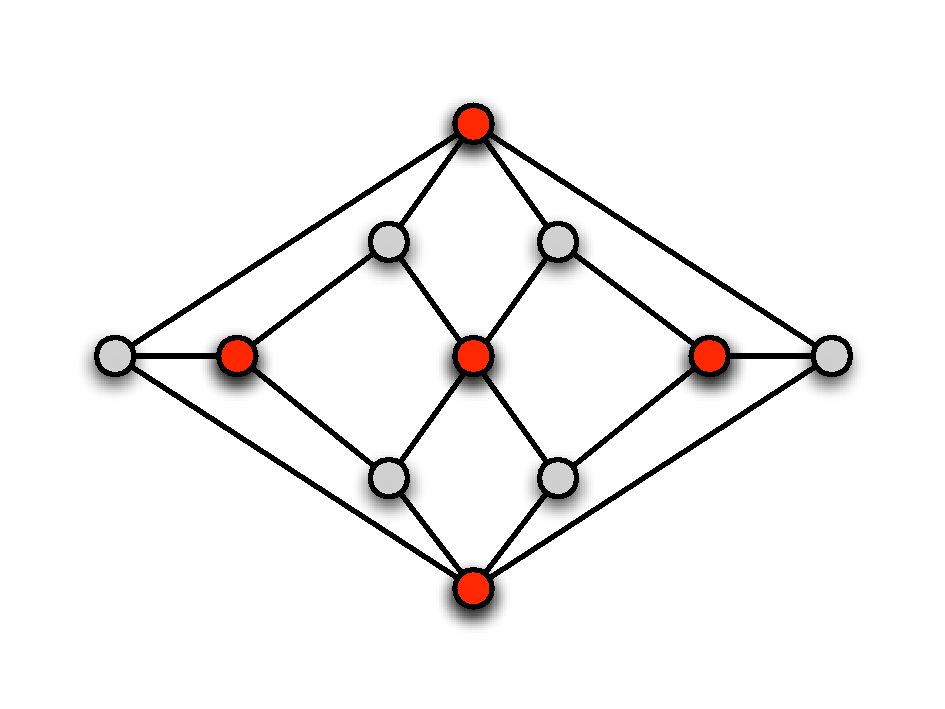
\includegraphics[width=10cm]{pic1.pdf}
\end{center}
\caption{Herschelov graf, vektorska grafika.}
\label{pic1}
\end{figure}
Pa res lahko vključimo slike katerihkoli formatov? Žal ne. Programski paket \LaTeX\ lahko uporabljamo v več dialektih. Ukaz {\tt latex} ne mara vključenih slik v formatu Portable Document Format {\tt .pdf}, ukaz {\tt pdflatex} pa ne prebavi slik v Encapsulated Postscript Formatu {\tt .eps}. 
Strnjeno v Tabeli~\ref{tbl:1}.

\begin{table}
\begin{center}
\begin{tabular}{l|ccc}
ukaz/format & {\tt .pdf} & {\tt .eps} & ostali formati \\ \hline
{\tt pdflatex} & da & ne & da \\
{\tt latex}   & ne & da  & da
\end{tabular}
\end{center}
\caption{}
\label{tbl:1}
\end{table}

Nasvet? Odločite se za uporabo ukaza {\tt pdflatex}. Vaš izdelek bo brez vmesnih stopenj na voljo v {.pdf} formatu in ga lahko odnesete v vsako tiskarno. Če morate na vsak način vključiti sliko, ki jo imate v {\tt .eps} formatu, jo vnaprej pretvorite v alternativni format, denimo {\tt .pdf}.

Včasih se da v okolju za uporabo programskega paketa \LaTeX\ nastaviti na kakšen način bomo prebavljali vhodne dokumente. Spustni meni na Sliki~\ref{pic2} odkriva uporabo \LaTeX{}a v njegovi pdf inkarnaciji --- {\tt pdflatex}.
\begin{figure}
\begin{center}

\includegraphics[width=10cm]{pic2.png}
\end{center}
\caption{Kateri dialekt uporabljati?}
\label{pic2}
\end{figure} 

Vključena Slika~\ref{pic2} je seveda bitna.

Kaj pa stran iz študentskega referata?\label{pp}
Tudi njo lahko vključimo v dokument. Toda ne kot plovko.
 



\begin{thebibliography}{99}
\label{bibliografija}

\bibitem{lf} L.\ Fortnow, ``Viewpoint: Time for computer science to grow up'',
{\it Communications of the ACM}, št.\ 52, zv.\ 8, str.\ 33--35, 2009.
\bibitem{dk1} D.\ E.\ Knuth, P. Bendix. ``Simple word problems in universal algebras'', v zborniku: Computational Problems in Abstract Algebra (ur. J. Leech), 1970, str. 263--297.
\bibitem{lat} L.\ Lamport. {\it LaTEX: A Document Preparation System}. Addison-Wesley, 1986.
\bibitem{bib} O.\ Patashnik (1998) \BibTeX{}ing. 
Dostopno na:\\ http://ftp.univie.ac.at/packages/tex/biblio/bibtex/contrib/doc/btxdoc.pdf
\bibitem{licence} licence-cc.pdf. Dostopno na: 

\end{thebibliography}


\end{document}

